\documentclass[11pt,a4paper]{ivoa}
\input tthdefs

\newcommand{\xtype}[1]{\texttt{#1}}
\newcommand{\ucd}[1]{\texttt{#1}}

\usepackage{listings}
\lstloadlanguages{XML,sh}
\lstset{flexiblecolumns=true,basicstyle=\small,tagstyle=\ttfamily}
\usepackage[utf8]{inputenc}
\usepackage{todonotes}
\usepackage{textcomp}
\usepackage{float}
\usepackage{lscape}
\usepackage{longtable}

\title{IVOA Obscore Extension for Visibility data}

\ivoagroup{Data Model Working Group}

\author{Fran\c cois Bonnarel}
\author{Mireille Louys}
\author{Mark Kettenis}
\author{Mark Lacy}
\author{Mattia Mancini}
\author{Yan Grange}
\author{Alan Loh}
\author{Baptiste Cecconi}

\editor{Fran\c cois Bonnarel}

\previousversion{}

       


\begin{document}

\begin{abstract}
This is a proposed extension to the Obscore specification for description of visibility data.
\end{abstract}

\section*{Acknowledgments}

The authors would like to thank all the participants in DM-WG and Radioastronomy-IG discussions 
for their ideas, critical reviews, and contributions to this document.
We acknowledge also the support of ESCAPE (European Science Cluster of Astronomy
and Particle Physics ESFRI Research Infrastructures) funded by the EU Horizon
2020 research and innovation program (Grant Agreement no 824064).
% are there other grants from partners to mention here?

\section{Introduction}


ObsCore specification \citep{std:OBSCORE} defines both a minimal datamodel to describe datasets 
and a table consistent with the model which can be served by TAP services. It has been successful 
to define a lot of data discovery services in astronomy.

The emergence of the Radioastronomy Interest Group in the IVOA in April 2020 confirmed the strong 
interest of the radio astronomy community to distribute their data in the VO. Many teams now 
distribute their data using VO standards\footnote{https://ivoa.net/documents/Notes/RadioVOImp/index.html}. 
While reduced radio data products, such as images or spectral cubes, %(and single dish data - {\it is that true ?} ) 
are mostly covered by the ObsCore model, the lower level observational data 
(interferometric visibilities) require additional description parameters. This was already exposed 
in 2010 when Anita Richards wrote a note called "Radio interferometry data in the VO" 
\footnote{https://wiki.ivoa.net/internal/IVOA/SiaInterface/Anita-InterferometryVO.pdf} which is 
still worth reading. The current specification tries to cover the needs exposed in this note. 
% Mireille an attempt to widen the scope ??
With the expansion of large radio astronomy projects such as LOFAR, NenuFAR, the future SKA, etc. 
and the emergence of interesting research topics matching data in all electromagnetic regimes, the 
Virtual Observatory framework can facilitate a wider access to radio data for experts and 
non-specialists radio astronomers in order to support collaborations in multi-wavelength, 
multi-messenger astronomy. 

%mireille:
% the needs for today as explored in recent meetings in Escape framework can also be summarized here
% add a short paragraph here
Although the interferometry data are nowadays dominant in radio field, similar issues occur for 
optical interferometry data. The extension we are defining here is valid for both domains.  


\begin{figure}[H]
\centering

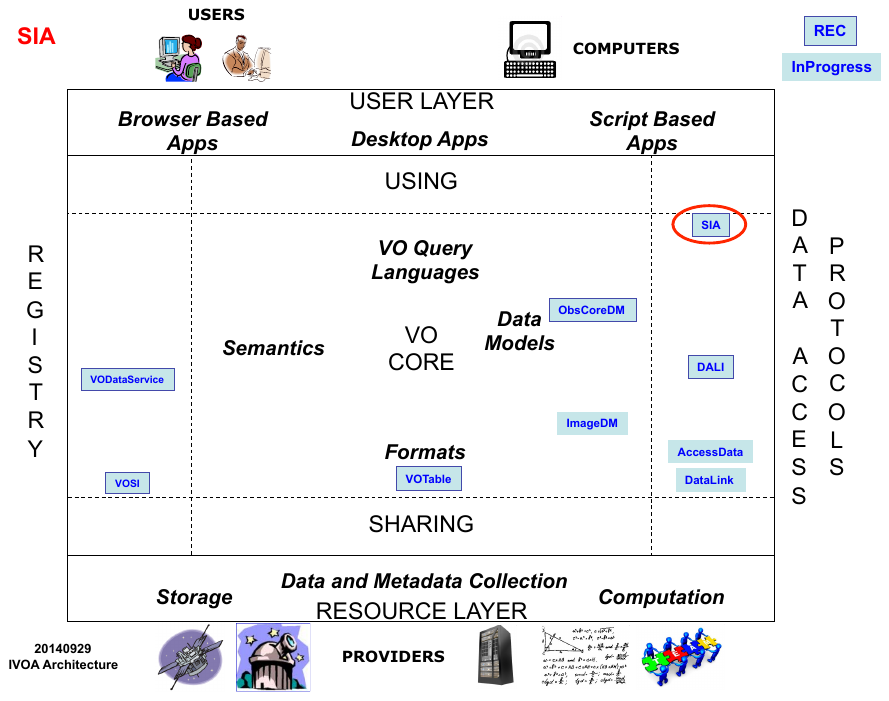
\includegraphics[width=0.9\textwidth]{archdiag.png}
\label{fig:architecture}
\end{figure}

% Mireille : it seems this is not the good diagram but the one of SIA 
% change architexture diag

%The role of this Visibility ObsCore extension in the IVOA is very close to ObsCore itself. It's only a fine grain improvement of this specification. 
% Mireille's  suggestion 
The scope of this Visibility ObsCore extension in the IVOA is very close to ObsCore itself. 
Its goal is to add new specific features to the existing ObsCore metadata tables and expose 
them in the ObsTAP TAP\_SCHEMA. 

\section{Visibility data specificities from the Data Discovery point of view}
\label{sec:specificities}

Visibility data are sets of complex numbers corresponding to the amplitude and phase 
of correlation coefficients measured between pair of antennas (i.e., a baseline), at 
a given time, a given wavelength or polarisation. The visibility data are a sparse 
representation of the observed sky. The visibility data sets can be processed to obtain 
interferometric images, through inverse Fourier algorithms. Each visibility measurement 
corresponds to an interferometric fringe system on the sky. 

The imaging algorithms include a calibration step allowing to set the center of the 
reconstructed image, setting this direction as a phase reference. The visibilities
are then usually represented in a spatial frequency plane, called the \emph{uv} plane, 
whose orientation is perpendicular to phase reference direction. The instantaneous PSF 
(Point Spread Function) of an interferometer is the Fourier transform of all baselines 
sampled in the \emph{uv} plane. Hence, the quality of the reconstructed images are 
directly related to the set of baselines used for the measurements.

Visibility data are usually organised as sets of matrices for various phase references
(i.e., pointing, or fields) and configuration of the baselines, such as their
distances and orientations. Such matrices may or may not be regularly sampled in time, 
wavelength and polarisation.
    
%How can the ObsCore parameters describe the characterization of these observations? 
As for any other data product described with ObsCore, the description may be split into
several records in the ObsCore table, when ObsCore parameters cannot represent the 
variety of the data product coverage (e.g., if there are several observed ``fields'', 
requiring different s\_ra and s\_dec value, or various groups of spectral bands, etc.) 

We consider that consistent ObsCore records as described above defines datasets with 
a dataproduct type set to ``visibility''.

On the lower end of the radio spectrum, radio astronomers generally make use of 
frequencies for designating the spectral ranges of their observation. The standard 
ObsCore attributes em\_min em\_max  are in wavelength and are not really convenient. 
That's why we should also provide their translation into frequencies. 
        
Moreover visibility data show some dependency of the spatial field of view and resolution 
with wavelength. Generally only a typical value for these two numbers can be given. It is 
noticeable that this is the case for any measuring system allowing a large interval of 
$\lambda/D$ (where $\lambda$ and $D$ are the wavelengths and the measuring system
aperture scale). 

Contrary to what occurs with direct imaging observations, the PSF of the interferometer
is filtering spatial scales (large scales, when the small baselines are insufficiently 
sampled; and vice versa for small scales with long baselines).
For large spectral ranges, the variations of the field of view and the spatial resolution 
along the axis may become so large that the typical value cannot be sufficient to 
characterize the dataset. Ranges of values for such parameters are required to accurately 
describe such datasets.

The quality of the data strongly depends from the distribution of the visibility measurements 
in the uv plane : the more complete the uv sampling plane, the better the reconstructed image. 
The uv plane distribution can be characterized by several numbers. 
The minimal and maximum distance between measurements in the uv plane provide assessments for 
spatial resolution and largest angular scale. 
Beside this a uv plane filling factor of the distribution will allow to predict the quality 
of reconstruction of the image in the distance plane (sky).
Eventually, the ellipticity of the distribution is a measure of the distortions that can 
affect the reconstruction.

Radioastronomers also check the quality of the visibility data by looking at some maps of 
the data structure. The uv coverage map can show how complete and regular is the sampling in 
the \emph{uv} plane and give an hint of resolution and maximum angular scale. 
The visualisation of the dirty beam, which is the Fourier transform of the \emph{uv} sampling 
function gives an hint of the intrinsic quality of possible reconstruction, as maps they are 
not queriable. So it is questionable if links to these maps are to be exposed in the extension 
table or only via a DataLink service. 

If none of these \emph{uv} characterization features are available to be exposed in the service 
we can still predict ranges of some of those by using some kind of facility description.  
Important features are the antenna diameter (or maximum antenna diameter), the number of 
antennae and the minimum and maximum distance between antennae of the array.

\section{ObsCore attributes definition valid for visibility data}
\label{sec:ObsCoreVisDef}

%Some mandatory or optional parameters will have peculiar estimation for visibility data.
For visibilities some of the definitions on Obscore datamodel elements need to be adjusted 
to fitthe peculiarity of medata for datasets partition, uv space, etc.

\subsection{obs\_id}

Astronomers usually know what they identify as a single observation : a complex set of 
measurements made in a given sequence of time. obs\_id should define unambiguously each 
observation.

\subsection{obs\_publisher\_did}

Visibility data observations can be split in several subparts with homogeneous spatial, 
time, spectral coverage intervals, spectral resolution, etc. Each part can be described by 
a single ObsCore dataset and has its own obs\_publisher\_did. It has to be unique in the 
Virtual Observatory domain.

\subsection{s\_fov}
\label{sec:fov}

A typical value for the field of view size will be given by $\lambda / D$ where $\lambda$ 
is the mid value of the spectral range and D is the largest diameter of the array antennae or 
telescopes.
 
\subsection{s\_resolution}
\label{sec:res}

A typical value for the spatial resolution will be given by $\lambda / L$ where $\lambda$ 
is the mid value of the spectral range and L is the longest distance in the \emph{uv} plane. 

\subsection{s\_region}

This shape will be the typical contour of the detectable beam. Of course it cannot be accurate. 

\subsection{o\_ucd}

In the case of visibility data the "observable" is a complex number representing Fourier 
coefficients of the image Fourier transform. Its UCD string is \emph{stat.fourier}. 

\subsection{t\_exptime}
TBC

\subsection{t\_resolution}
TBC 

\section{ObsCore extension for visibility data}

Table \ref{tab:ExtensionAtt} shows the %additional 
parameters we propose to add to ObsCore in order to better describe visibility data.
Two options can be considered in the TAP or SIA services descriptions: 
\begin{itemize}
\item adding the new data model elements directly into the main ObsCore table
\item providing an extra table for these, named ivoa.visibilities for instance,  which will 
be joined to the main table. 
\end{itemize}

\subsection{spatial parameters}

The s\_maximum\_angular\_scale is estimated as $\lambda/l$ where $\lambda$ is the typical 
wavelength and l is the smallest distance in the uv plane. s\_fov\_min, s\_fov\_max, 
s\_resolution\_min, s\_resolution\_max are estimated like the typical values (see subsections 
\ref{sec:fov} and \ref{sec:res} ) where $\lambda$ is replaced by the minimum and maximum 
wavelength of the spectral ranges


\subsection{uv parameters}

%uv\_distance\_min and uv\_distance\_max are straigthforward.
uv\_distance\_min and uv\_distance\_max are evaluated by fitting an ellipse on the 
visibilities present in the uv plane.

% Mireille but still for the spec it is good to redefine them here
To compute the ellipse's eccentricity of the UV distribution a principal component analysis 
(PCA) with 2 components is performed over the data points sampling the UV plane to select the 
main axis of data scattering. 
The first component is used to rotate the distribution of UV in a way that the major variation 
of the distribution is leaning towards the $x$ axis of a bi dimensional $xy$ Cartesian plane. 
The major axis length and the minor axis length of the ellipse are therefore defined as the 
semi distance between the most positive point along the $x$/$y$ axis and the most negative point 
among the $y$ axis. For instance, if the range of the rotated UV will cover on the $x \in [-10, 
10]$ the major axis distance would be 10, a similar procedure is done on the y axis. This 
procedure allows the definition of the \emph{UV} distribution eccentricity:

uv\_distribution\_exc) computed as follows:
\begin{equation}
uv\_distribution\_exc = \sqrt{1-\frac{b^2}{a^2}}
\end{equation}
where a is the major axis length and b is the minor axis length.
The filling factor of the UV plane (hereafter uv\_distribution\_fill) is computed as the average 
number of samples found in a $N^{uv}_{samples}$x$N^{uv}_{samples}$ equi-spaced grid enclosing the 
rotated ellipse. In formulas, the boundaries of a cell (i,j) are defined by the boundaries
\begin{equation}
u \in [u_{min} + \frac{u_{max} - u_{min}}{N^{uv}_{samples}} \cdot i , u_{min} + \frac{u_{max} - 
u_{min}}{N^{uv}_{samples}} \cdot (i + 1)]
\end{equation} 
and
\begin{equation}
v \in [v_{min} + \frac{v_{max} - v_{min}}{N^{uv}_{samples}} \cdot j , v_{min} + \frac{v_{max} - 
v_{min}}{N^{uv}_{samples}} \cdot (j + 1)]
\end{equation} 
where $u_{max}$/$v_{max}$ are the respective maximum u/v of the \emph{uv} sample and 
$u_{min}$/$v_{min}$ is the minimum u/v of the \emph{uv} sample.

Given the above boundaries the number of samples within a cell (i,j) will be $n^{uv}_{i,j}$ 
and uv\_distribution\_fill will be then computed as 
\begin{equation}
uv\_distribution\_fill = \frac{\sum^{N^{uv}_{samples}}_{i=1} \sum^{N^{uv}_{samples}}_{j=1} 
n^{uv}_{i,j} }{(N^{uv}_{samples}) ^ 2},
\end{equation}

in the preliminary analysis $N^{uv}_{samples} = 1000$.


% Mireille: moved time param below uv space because uv plane deals with spatial features 

\subsection{time parameters}

t\_exp\_min and t\_exp\_max are added because of strong variation in the individual timestamps 
duration.
\subsection{instrumental parameters}

They all give a predefined raw idea of resolution, field of view, maximum angular scale and 
sampling quality.

\subsection{uv coverage and dirty beam map}

These uv\_coverage\_map and s\_resolution\_beam\_dirty parameters are  intended to be url to 
files containing these maps. 
Implementers may want to avoid adding url columns to the ObsCore table. 

In that case DataLink \citep{std:DataLink} may provide a solution. The semantics FIELD in the 
\{link\} response  will contain \#auxiliary  for links to this map while  the content\_qualifier 
FIELD could contain the utype defined here in this ObsCore extension.


\section{How to implement the extension in a TAP service}

The ObsCore extension for visibility data described above SHOULD not be added to the main ObsCore table. An extension table called "visibilityobscore" SHOULD be added to the same schema instead. The two tables will be joigned in an extended ObsTAP ADQL query. A single dataset in each observation will be associated to a single row in ObsCore. It will be identified by a unique obs\_publisher\_did. This obs\_publisher\_did can be used as a foreign key to join the main table and the extension

In the registry, the service capability will contain the ObsCore Model element an the visisbilityobscore Model element   and the visibilityobscore table will be described in the tableset of the service together with obscore.  




        
\begin{landscape}
\begin{longtable}{l  p{4cm} p{4cm} p{4cm} l l}
\sptablerule
\textbf{column name}&\textbf{definition}&\textbf{utype}&\textbf{ucd}&\textbf{unit}\cr
\sptablerule
\sptablerule
\texttt{ s\_resolution\_min}&\texttt{ Angular resolution, longest baseline and  max frequency dependant}&{ Char.SpatialAxis.\newline Resolution.Bounds.\newline Limits.LoLim}&{pos.AngResol;stat.min}&{arcsec}\cr
\sptablerule
\texttt{s\_resolution\_max}&\texttt{Angular resolution, longest baseline and min frequency dependant}&\texttt{Char.SpatialAxis.\newline Resolution.Bounds.\newline Limits.HiLim}&{pos.AngResol;stat.max}&arcsec\cr
\sptablerule
\texttt{s\_fov\_min}&\texttt{field of view diameter,  min value, max frequency dependant}&\texttt{Char.SpatialAxis.\newline Coverage.Bounds.\newline Extent.LowLim}&{phys.angSize;instr.fov;\newline stat.min}&deg\cr
\sptablerule
\texttt{s\_fov\_max}&\texttt{field of view diameter,  max value, min frequency dependant}&\texttt{Char.SpatialAxis.\newline Coverage.Bounds.\newline Extent.HiLim}&{phys.angSize;instr.fov;\newline stat.max}&deg\cr
\sptablerule
\texttt{s\_maximum\_angular\_scale}&\texttt{maximum scale in dataset, shortest baseline and  frequency dependant}&\texttt{Char.SpatialAxis.\newline Resolution.Scale.\newline Limits.HiLim}&{phys.angSize;stat.max}&arcsec\cr
\sptablerule
\texttt{f\_min}&\texttt{spectral coverage min in frequency}&\texttt{Char.SpectralAxis.\newline Coverage.Bounds\newline Limits.LoLim}&{em.freq;stat.min}&Mhz\cr
\sptablerule
\texttt{f\_max}&\texttt{spectral coverage max in frequency}&\texttt{Char.SpectralAxis.\newline Coverage.Bounds\newline Limits.HiLim}&{em.freq;stat.max}&Mhz\cr
\texttt{t\_exp\_min}&\texttt{minimum integration time per sample}&\texttt{Char.TimeAxis.\newline Sampling.Extent\newline LoLim}&{time.duration;obs.exposure;\newline stat.min}&s\cr
\sptablerule
\texttt{t\_exp\_max}&\texttt{maximum integration time per sample}&\texttt{Char.TimeAxis.\newline Sampling.Extent\newline HiLim}&{time.duration;obs.exposure;\newline stat.max}&s\cr
\sptablerule
\texttt{uv\_distance\_min}&\texttt{minimal distance in uv plane}&\texttt{Char.UVAxis.\newline  Coverage.Bounds.\newline Limits.LoLim}&stat.fourier;pos;stat.min&m& \cr
\sptablerule
\texttt{uv\_distance\_max}&\texttt{maximal distance in uv plane}&\texttt{Char.UVAxis.\newline  Coverage.Bounds.\newline Limits.LoLim}&stat.fourier;pos;stat.max&m \cr
\sptablerule
\texttt{uv\_distribution\_exc}&\texttt{excentricity of uv distribution}&\texttt{Char.UVAxis.\newline  Coverage.Bounds.\newline Excentricity}&stat.fourier;pos& \cr
\sptablerule
\texttt{uv\_distribution\_fill}&\texttt{filling factor of uv distribution}&\texttt{Char.UVAxis.\newline  Coverage.Bounds.\newline FillingFactor}&stat.fourier;pos& \cr
\sptablerule
% mireille here for antennae features , it is clear it belongs to instrument. 
%Not useful to use the term in the name .
%\texttt{instrument\_ant\_number}&\texttt{number of antennae in array}&\texttt{Provenance.ObsConfig.\newline Instrument.Array.\newline AntNumber}&instr.baseline;meta.number& \cr
%\sptablerule
\texttt{ant\_number}&\texttt{number of antennae in array}&\texttt{Provenance.ObsConfig.\newline Instrument.Array.\newline AntNumber}&instr.baseline;meta.number& \cr
\sptablerule
% same for all antenae features
\texttt{instrument\_ant\_min\_dist}&\texttt{minimum distance between antennae in array}&\texttt{Provenance.ObsConfig.\newline Instrument.Array.\newline MinDist}&instr.baseline;stat.min&m \cr
\sptablerule
\texttt{instrument\_ant\_max\_dist}&\texttt{maximum distance between antennae in array}&\texttt{Provenance.ObsConfig.\newline Instrument.Array.\newline MaxDist}&instr.baseline;stat.max&m \cr
\sptablerule
\texttt{instrument\_ant\_diameter}&\texttt{diameter of antennae in array}&\texttt{Provenance.ObsConfig.\newline Instrument.Array.\newline Diameter}&instr&m \cr
\sptablerule
\texttt{uv\_distribution\_map}&\texttt{uv distribution map}&\texttt{Char.UVAxis.\newline  Sampling.\newline Sensitivity.Map}&stat.fourier;pos& \cr
\sptablerule
\texttt{s\_resolution\_beam\_dirty}&\texttt{dirty beam}&\texttt{Char.SpatialAxis.\newline Resolution.\newline Variability.DirtyBeam.\newline Map}&{pos.AngResol}&\cr

\caption{ObsCore visibility data extension parameters}
\label{tab:ExtensionAtt}
\end{longtable}
\end{landscape}


\bibliography{ivoatex/ivoabib}

\end{document}
